\section{Introduction}
%Approximate inference in probabilistic models with continuous latent variables seeks to model intractable posterior distributions of latent codes given observed data. 
Stochastic variational inference (SVI) methods provide an appealing way of scaling probabilistic modeling to large scale data.
These methods transform the problem of computing an intractable posterior distribution to finding the best approximation within a class of tractable probability distributions \cite{hoffman2013stochastic}.
Using tractable classes of approximate distributions, \eg, mean-field, and Bethe approximations, facilitates efficient inference, at the cost of limiting the expressiveness of the learned posterior. 
%However, it also limits the expressivity of the approximate posterior, and even in the asymptotic regime learning may be unable to produce samples from the true posterior when using such strong assumptions \cite{blei2017variational}. 

In recent years, the power of these SVI methods has been further improved by employing {\em normalizing flows}, which greatly increase the flexibility of the approximate posterior distribution. 
%Recent work on {\em normalizing flows} alleviates this modeling bottleneck.
Normalizing flows involve learning a series of invertible transformations, which are used to transform a sample from a simple base distribution to a sample from a richer distribution \cite{rezende2015variational}. 
Indeed, flow-based posteriors enjoy many advantages such as efficient sampling, exact likelihood estimation, and low-variance gradient estimates when the base distribution is reparametrizable, making them ideal for modern machine learning problems.
There have been numerous advances in normalizing flow construction in Euclidean spaces from RealNVP \cite{dinh2016density}, NAF \cite{huang2018neural}, and FFJORD \cite{grathwohl2018ffjord} to name a few.

\begin{figure}
    \centering
    \vspace{-10pt}
    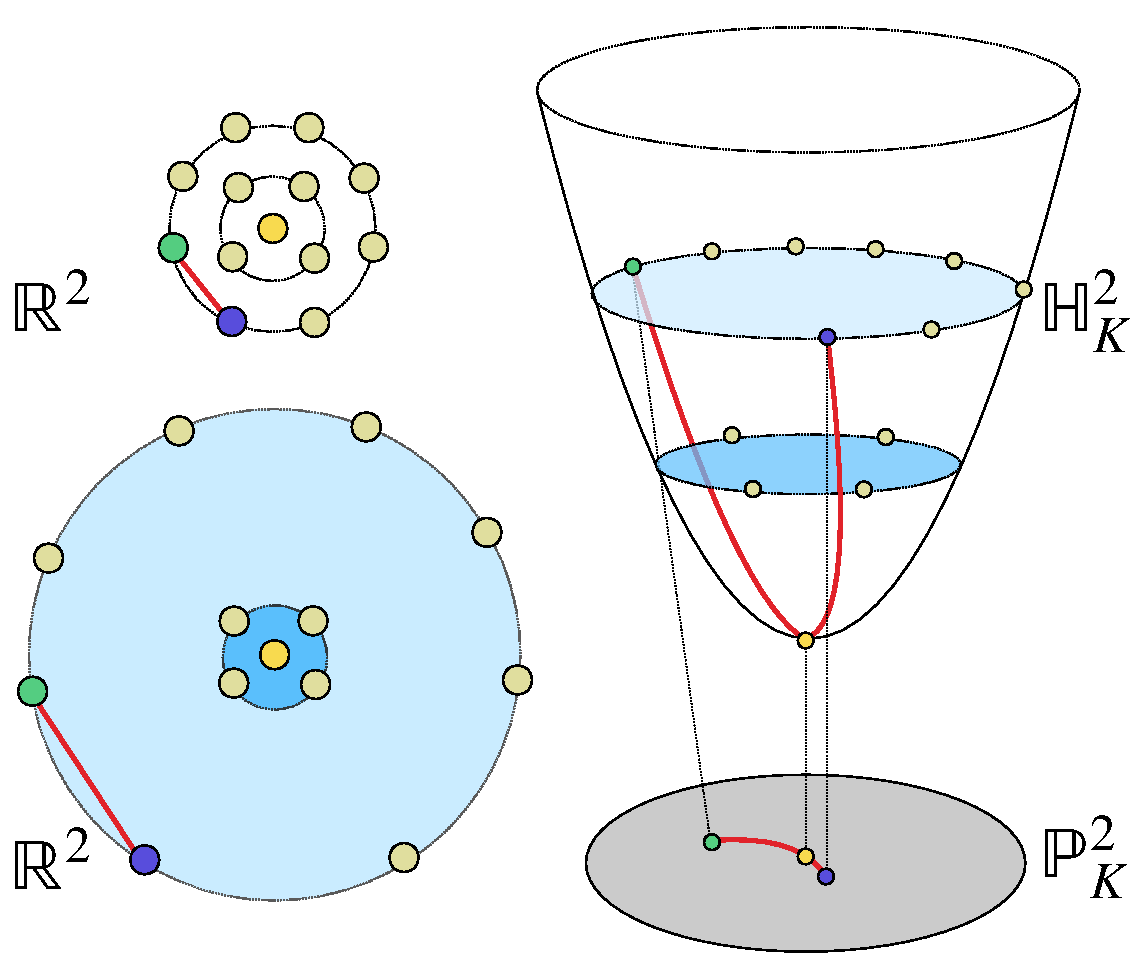
\includegraphics[width=0.9\linewidth]{explanatory_fig.pdf}
    \vspace{-10pt}
    \caption{The shortest path between a given pair of node embeddings in $\mathbb{R}^2$ and hyperbolic space as modelled by the Lorentz model $\mathbb{H}^2_K$ and Poincar\'e disk $\mathbb{P}^2_K$. Unlike Euclidean space, distances between points grow exponentially as you move away from the origin in hyperbolic space, and thus the shortest paths between points in hyperbolic space go through the origin, giving rise to hierarchical, tree-like structure. }
    \vspace{-10pt}
    \label{fig:explanatory_fig_1}
\end{figure}

However, current normalizing flows are restricted to Euclidean space, and as a result, these approaches are ill-equipped to model data with an underlying hierarchical structure. %and fail to incorporate structural inductive biases.
%As a result, the learning problem often needs to \textit{rediscover} structure---such as hierarchy---that is known {\em a priori}.
%While  they fail to incorporate known structure in data burdening the learning problem as it needs to \textit{rediscover} structure that is known apriori. 
Many real-world datasets, such as ontologies, social networks, sentences in natural language, and evolutionary relationships between biological entities in phylogenetics exhibit rich hierarchical or tree-like structure.
Hierarchical data of this kind can be naturally represented in hyperbolic spaces, \ie, non-Euclidean spaces with constant negative curvature (Figure \ref{fig:explanatory_fig_1}). 
But Euclidean normalizing flows fail to incorporate these structural inductive biases, since Euclidean space cannot embed deep hierarchies without suffering from high distortion \cite{sarkar2011low}. Furthermore, sampling from densities defined on Euclidean space will inevitability generate points that do not lie on the underlying hyperbolic space. 
%Intuitively, this occurs due to a fundamental geometric limitation of Euclidean spaces.
%Hierarchies (i.e, trees) generally grow exponentially as their depth increases, and the homogeneous structure of Euclidean space is unable to embed such exponential growth. 

%embed deep hierarchies
%The main challenge of probabilistic modeling of hierarchical data is that conventional Euclidean spaces are ill-equipped to embed deep hierarchies
%observational data to continuous latent variables without suffering from high distortion \cite{sarkar2011low}. 
%Intuitively, this occurs due to a fundamental geometric limitation of Euclidean spaces.
%Hierarchies (i.e, trees) generally grow exponentially as their depth increases, and the homogeneous structure of Euclidean space is unable to embed such exponential growth. 
%Indeed, if an underlying data distribution lies on a hyperbolic manifold, performing density estimation in Euclidean space 

%Recently, hyperbolic spaces have been proposed as an alternative to embedding hierarchical data due to their attractive geometric properties. 
%For example, hyperbolic spaces can be thought of as the continuous analogs of trees and can be used to embed trees with arbitrarily low distortion. 

\xhdr{Present work} 
To address this fundamental limitation, we present the first extension of normalizing flows to hyperbolic spaces. 
%Our work answer the question: how can we learn rich probability distributions over hyperbolic latent variables? 
%Currently, there are no existing approaches to extend normalizing flows to hyperbolic spaces
%Despite the known importance of leveraging hyperbolic spaces for modeling hierarchical data \cite{nickel2018learning}, there are no existing approaches for flexible density estimation on hyperbolic spaces. 
Prior works have considered learning models with hyperbolic parameters  \cite{liu2019hyperbolic,nickel2018learning} as well as variational inference with hyperbolic latent variables \cite{nagano2019wrapped,mathieu2019continuous}, but our work represents the first approach to allow flexible density estimation in hyperbolic space. 
%but the approximate posterior distribution is still limited due to the mean-field assumption. 
%In this work, we answer the following question: how can we learn rich probability distributions over hyperbolic latent variables? 
%using stochastic variational inference that better approximate true posteriors for hierarchical data?

%We appeal to the geometry of hyperbolic spaces and construct novel normalizing flows in the Lorentz model of hyperbolic geometry. 
To define our normalizing flows we leverage the Lorentz model of hyperbolic geometry and introduce two new forms of coupling, {\em Tangent Coupling} ($\mathcal{TC}$) and {\em Wrapped Hyperboloid Coupling} ($\mathcal{W}\mathbb{H}\mathcal{C}$). These define flexible and invertible transformations capable of transforming sampled points in the hyperbolic space. 
We derive the change of volume associated with these transformations and show that it can be computed efficiently with $\mathcal{O}(n)$ cost, where $n$ is the dimension of the hyperbolic space.
We empirically validate our proposed normalizing flows on structured density estimation, reconstruction and generation tasks on hierarchical data, highlighting the utility of our proposed approach. \cut{We find that using Wrapped Hyperbolic flows allows for a \red{\%XX} an aggregate absolute improvement over Euclidean flows.}

